\subsection{Graph Network Library}

Abstract (features, purpose)

Alternatives: DeepMind's, not chosen bc TF and we wanted to have full understanding and learning.

Overview of classes, internal structure, maybe more details on aforementioned features. General concept of generic classes and implementations done by the user. Some default implementations are provided

\begin{figure}\centering
    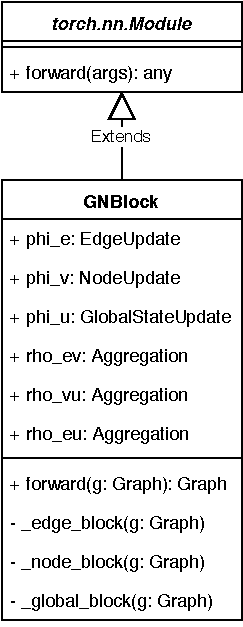
\includegraphics[scale=0.65]{resources/graphnets-block}
    \caption{Class diagram of the graph network library GNBlock class}\label{fig:classdiagramgnblock}
\end{figure}

\begin{figure}\centering
    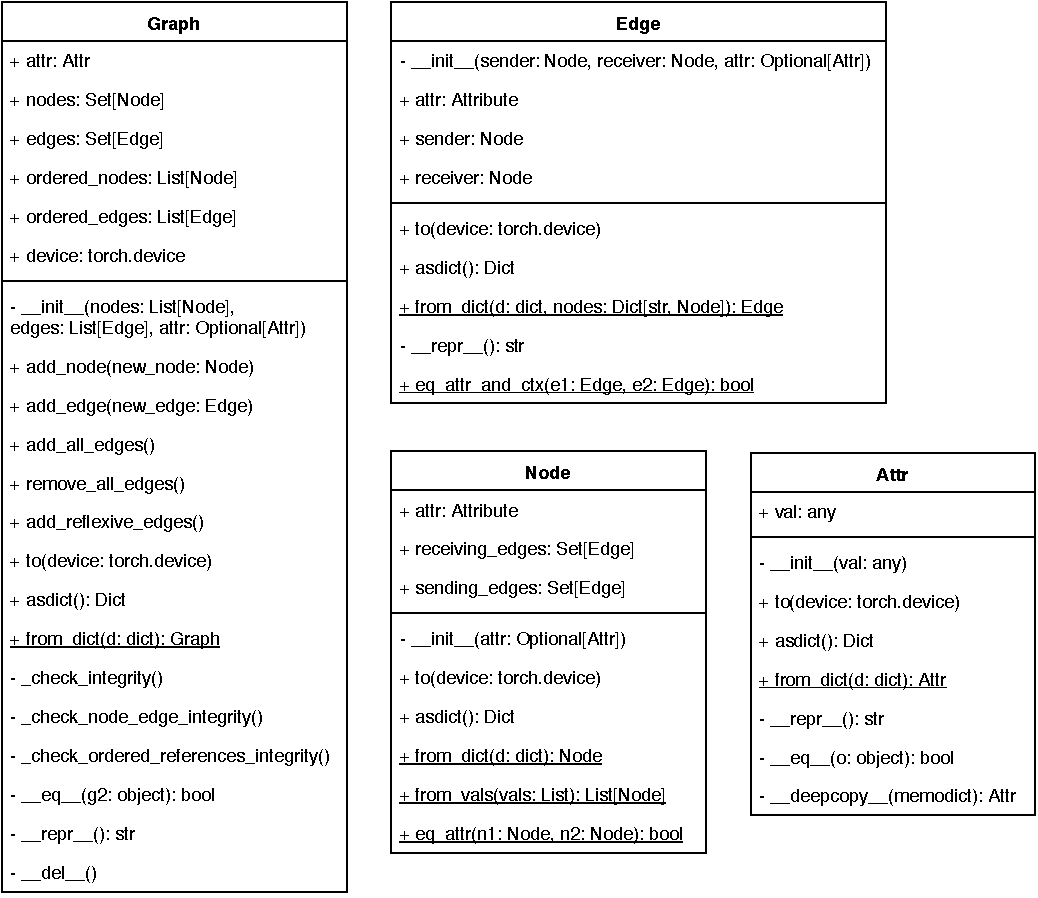
\includegraphics[scale=0.65]{resources/graphnets-datastructs}
    \caption{Class diagram of the graph network library data structure classes}\label{fig:classdiagramgndatastructs}
\end{figure}

\begin{figure}\centering
    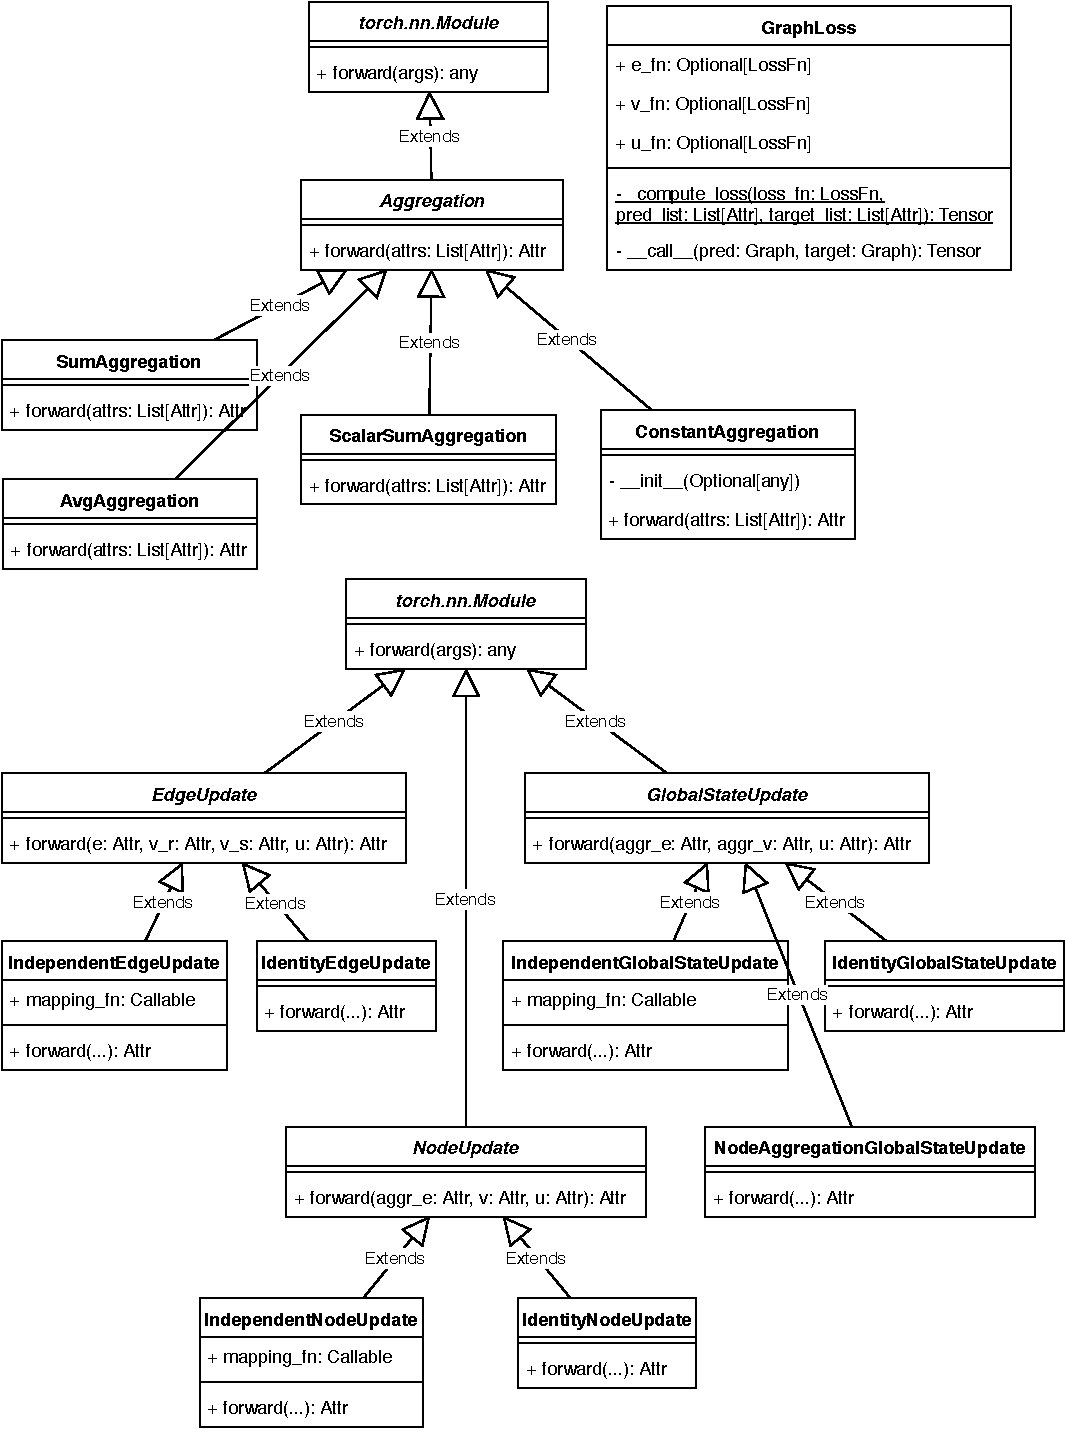
\includegraphics[scale=0.65]{resources/graphnets-functions}
    \caption{Class diagram of the graph network library aggregation functions, update functions, and graph loss class}\label{fig:classdiagramgnfunctions}
\end{figure}

Elaborate on each class and name details.

Future improvements: parallelize, CUDA ops, more default implementations
